\section{Query-based Federated Learning}
\label{sec:query}
\subsection{Overview}
\label{sec:query_overview}
Let us continue by establishing a sustainable open FL platform based on a query-based cooperation framework.
An overview of this platform is presented in Fig.~\ref{fig:query}, the desin philosophy behind this framework is to break the coupling between FL server and clients.
In the query-based FL systems, all traditional FL roles and components are maintained on an open model repository called Model Community. The Model Community privdes a one-stop ML models redistribution and reuse service, including model indexing, automatic batch model reuse, license management, privacy control and so on.
In addition to large-scale pretrained models like BERT~\cite{devlin2018bert}, BLOOM~\cite{scao2022bloom} with great generalization abilities, we also encourage individuals to upload their task-specific models trained on limited domain data to boost the knowledge mining within models, aka model mining~\cite{you2021workshop}.
The derivatives of model mining can learn representations from multiple domains, resulting in more promising performance that can be evaluated by platform users.
Furthermore, the contributors can release models under applicable licenses, granting them distribution control and legal protection of their intellectual property (IP).
In summary, the properties of query-based FL are:
(1) \textbf{Model Agnostic}, as there are no restrictions on the types and architectures of the models uploaded by users;
(2) \textbf{Contactless}, as communication channels need not be maintained; 
(3) \textbf{Community-powered}, whereby sharing models enrichs the entire community.

\begin{figure}[t]
  \centering
  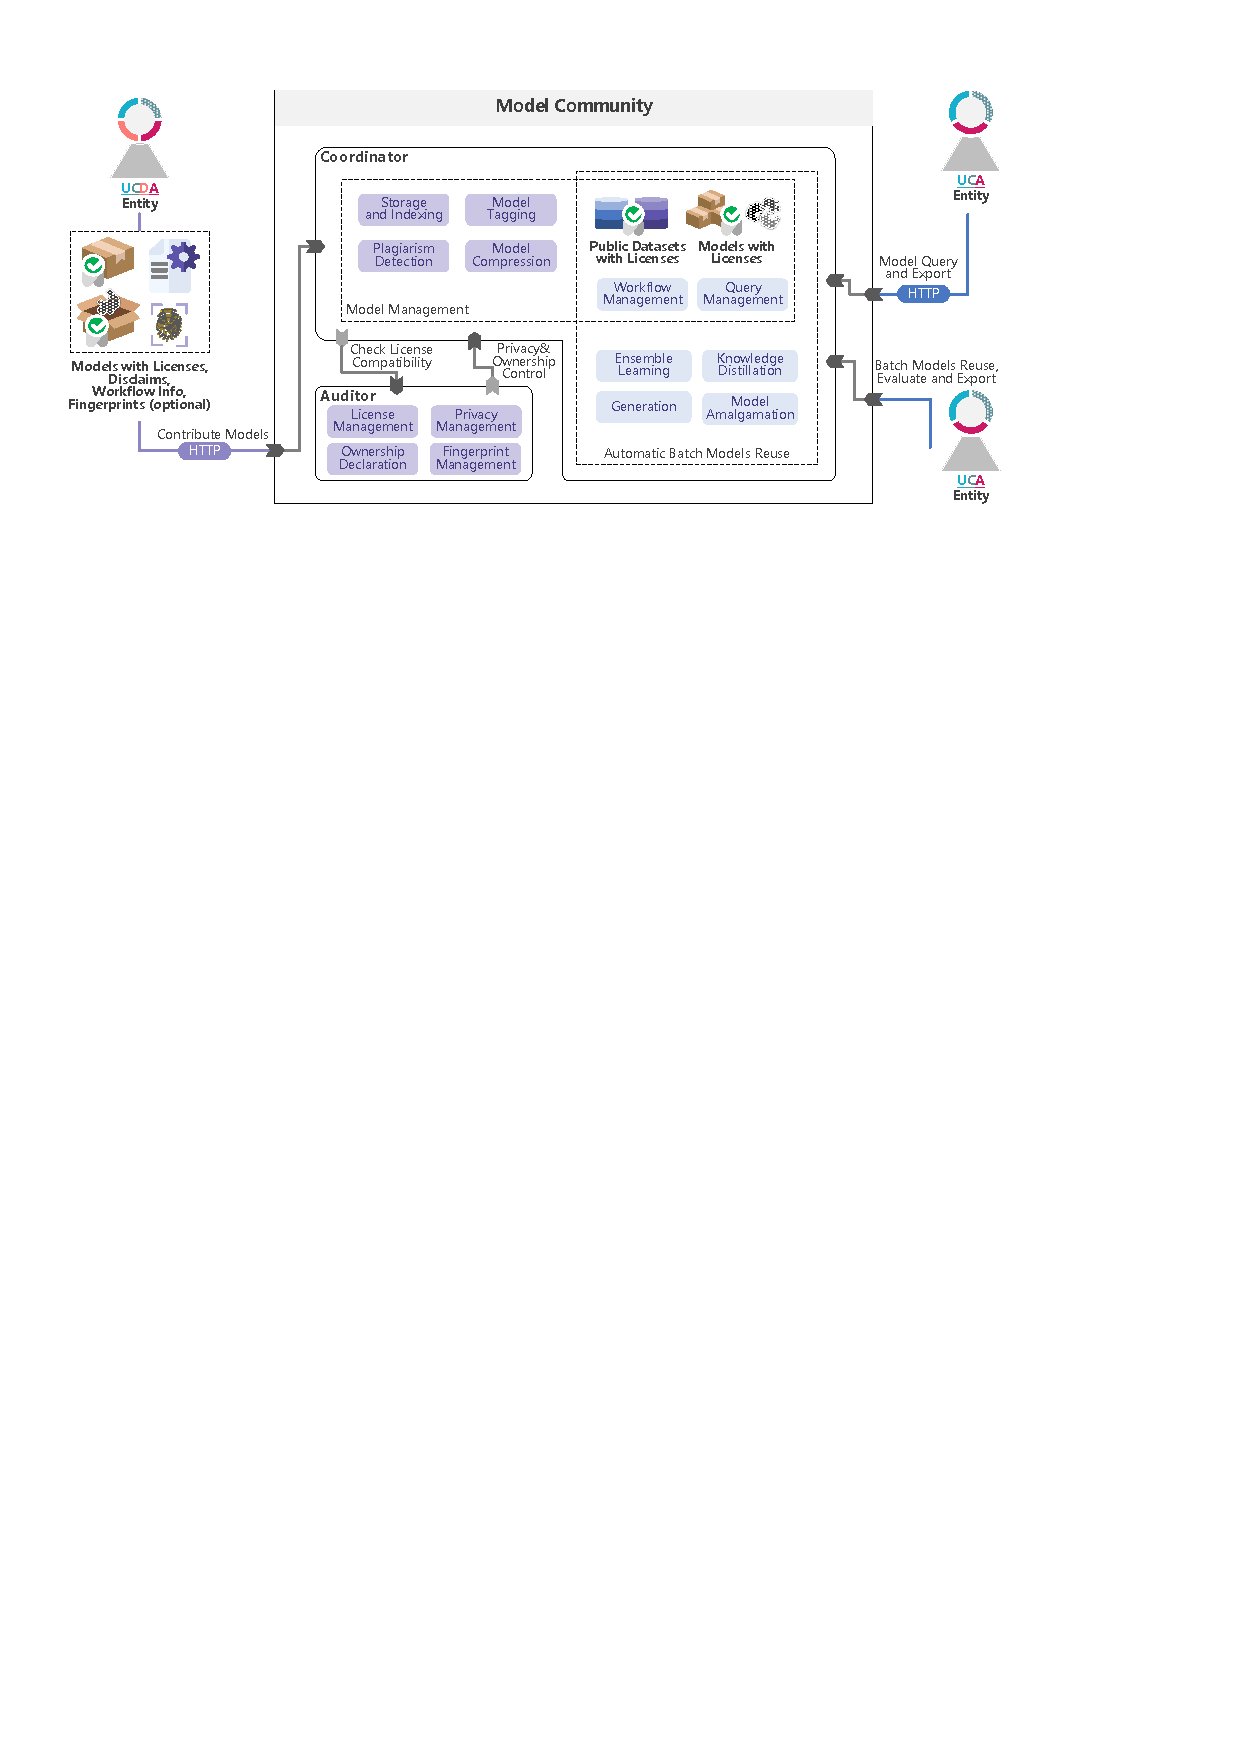
\includegraphics[width=\linewidth]{fig/query_frame.pdf}
  \caption{An overview of query-based FL systems. (U: model User, C: Coordinator, D: Data owner, A: Auditor)}
  \label{fig:query}
\end{figure}

Actually, we aim to advocate a novel SaaS~\cite{brereton1999future} ML platform with automatic batch model reuse integrated, which has potential to leverage the transportability of models to address previously unexplored ML problems.
Due to the high computational demands of deep learning, current ML platforms primarily concentrate on computing, for example, MaaS, MLaaS, FLaaS provide ML models deployment and development services to handle user-specified tasks\textsuperscript{\ddag{I-B}}.
On the other hand, there are several ML platforms provide open model search and download services. 
So, can we leverage leverage off-the-shelf public model repositories to build a query-based FL system?
Unfortunately, these sites are designed solely for sharing and are not suitable for more advanced functionalities such as model ensemble~\cite{jacobs1991adaptive} and knowledge distillation (KD)~\cite{hinton2015distilling}, and we will explain the reasons in the following section.

% Model Mining

\subsection{How to Query for Models}
\label{sec:how2query}
To establish a query-based FL platform, the first thing that comes to mind is how to query for models.
Unlike traditional ML model sharing repositories that mainly query for a specific model by name, it requires an efficiency approach to export a batch of target models that are ready for ensemble or distillation.
We summarized the filter conditions of existing DNNs sharing repositories\footnote{Hugging Face: \url{https://huggingface.co}; Model Zoo: \url{https://modelzoo.co}; Tensorflow Hub: \url{https://tfhub.dev}; NVIDIA NGC: \url{https://catalog.ngc.nvidia.com/models};  OpenVINO: \url{https://docs.openvino.ai/latest/model\_zoo.html}; Pytorch Hub: \url{https://pytorch.org/hub}} in TABLE.~\ref{table:repository}.
The prevailing method for querying models involves searching for the desired model by its name, used datasets, and the associated tasks.
For instance, one might search for the model name GPT~\cite{radford2019language}, models trained on the MNIST dataset~\cite{lecun2010mnist}, or models capable of performing image segmentation tasks.
However, this model retrieval method requires the users have a strong priori knowledge in data science, thus raising the barrier for knowledge mining within models.
As an example, there is no effective way to acquire a batch of image classfication models that contains the knowledge of \textit{lesser panda} for further distillation.
A compromise solution is to manually search the schema of each dataset one-by-one and subsequently search for models trained on those datasets.

As shown in TABLE.~\ref{table:repository}, most DNNs repositories are simply listing the description of input/output (e.g., NVIDIA NGC, OpenVINO) or even just present the source codes (e.g., Tensorflow Hub, Pytorch Hub).
This lack of unified convention for model input/output poses a challenge for query-based FL.
Additionally, most of DNNs repositories do not enable querying models by licenses, resulting in the cumbersome task of individually handling model licenses and ensuring compatibility among different licenses.
Hence, it is imperative to reconsider the design of DNNs repositories to enable quick identification of readily reusable models for knowledge aggregation. 
We further suggest following filter conditions for query-based FL: 1) Data Description; 2) Workflow and History; 3) Software Dependency; 4) Fairness and Robustness\textsuperscript{\ddag{II}}. %We leave the detailed reasons in Appendix~II.

%%% FACTsheet

\begin{table*}[t]
  \centering
  \caption{Filter conditions and characteristics of DNNs repositories. \cmark : Supported, \xmark : Unsupported, \textbf{!} : Information provided but unsearchable, listed in descending order by number of released models. (Accessed on January 17, 2024)}
  \label{table:repository}
  \footnotesize
  \begin{tabular}{|l|c|c|c|c|c|c|c|c|}
  \hline
  & \multicolumn{1}{l|}{DS Name} & \multicolumn{1}{l|}{Model Architecture} & \multicolumn{1}{l|}{Modality/Task} & \multicolumn{1}{l|}{Tag} & \multicolumn{1}{l|}{License} & \multicolumn{1}{l|}{Input-Output} & \multicolumn{1}{l|}{Batch Export} & \multicolumn{1}{l|}{\# of Models}\\ \hline
  Hugging Face & \cmark & \cmark & \cmark & \cmark & \cmark & \textbf{!} & \xmark & 470,263 \\ \hline
  Model Zoo & \cmark & \cmark & \cmark & \cmark & \xmark & \xmark & \xmark & 3,245 \\ \hline
  Tensorflow Hub & \cmark & \cmark & \cmark & \cmark & \textbf{!} & \textbf{!} & \xmark & 2,186 \\ \hline
  NVIDIA NGC & \textbf{!} & \cmark & \cmark & \cmark & \textbf{!} & \textbf{!} & \xmark & 680 \\ \hline
  OpenVINO & \textbf{!} & \cmark & \cmark & \xmark & \textbf{!} & \textbf{!} & \cmark & 277 \\ \hline
  Pytorch Hub & \textbf{!} & \cmark & \xmark & \xmark & \xmark & \textbf{!} & \xmark & 52 \\ \hline
  \end{tabular}
\end{table*}

The aforementioned filter conditions provide comprehensive coverage of the ML modeling process. 
However, there are additional requirements depending on the reuse mechanisms in the model retrieval side. 
For example, FedAvg~\cite{mcmahan2017communication} aggregates the local models weights element-wise, which requires full access to the models. 
In contrast, MoE~\cite{jacobs1991adaptive} only ensembles a batch of model outputs, so the individual models can remain blackboxes in this scenario.
So, in the context of software licenses or model licenses, the batch models reused by FedAvg should be released as source code, while those reused by MoE can be released as binary executable modules (e.g., dynamic linking).
The above distinction is crucial for ensuring that model reuse results meet the legal framework, and this has been overlooked in traditional FL.
We will expand on this topic in the following section.

\subsection{Legal Considerations in Batch Model Reuse}
\label{sec:how2reuse}
Once we have acquired a batch of models that can contribute to the new target task, the next step is to reuse the knowledge of these pre-trained models, i.e., transfer their knowledge from source domain to the target domain~\cite{pan2009survey}.
However, before deciding on how to reuse the model, it is important to ensure that the rights and permissions have been obtained. 
This may involve reviewing the terms and conditions of the licenses under which the models were released or obtaining permission from the original creators or copyright holders.
Therefore, in this section, we will not focus on the technical details of how to reuse models, which is already covered by many related surveys, such as Transfer Learning~\cite{pan2009survey}, Ensemble Leanring~\cite{zhou2012ensemble}, Domain Adaptation~\cite{wang2018deep}, Knowledge Distillation~\cite{wang2021knowledge}, Deep Generative Models~\cite{cao2022survey} and Model Fusion~\cite{ji2021emerging}.
Meanwhile, the specific model reuse techniques used are at the user's discretion, and the query-based FL platform is not bounded or restricted to any particular reuse method.
Innovatively, we study how to reuse batch of models, from the perspective of \textbf{legal compliance}.
%Therefore, the focus of this section is how to reuse batch of models, from the perspective of legal compliance.

The machine learning community benefits from the openness of ideas and code, and many high-impact ML conferences and journals encourage authors to publish their source code and dataset to research platforms like Papers With Code\footnote{https://paperswithcode.com} and Code Ocean\footnote{https://codeocean.com} to increase exposure and facilitate reproducibility.
To restrict the use of ML techniques for unethical purposes (i.e., Deepfakes~\cite{mirsky2021creation}) and protect the IP of creators, models are typically published under a license agreed upon by the licensor.
Here, we summarized the granted rights, restrictions and enforcements of licenses for ML models posted on Hugging Face in TABLE~\ref{tab:licenses}.
The following sections will provide a detailed survey of these licenses.


\begin{table*}[t]
  \centering
  \scriptsize
  \caption{Licenses for ML models available on Hugging Face with a focus on their rights, restrictions and enforcements, grouped by FOSS licenses, AI model licenses, free content or database licenses in descending order of number of models (GPL, BSD, LGPL, CC licenses with unspecified versions are excluded, the similar revisions are merged). \cmark : Permited or Required, \xmark : Not Permited or Not Required, \textbf{!} : Not Explicitly Permited, * : Copyleft License, $^{\dagger}$ : Public Domain License. Only the source code of the original work under AFL-3.0 or Artistic-2.0 is required to be disclosed. You may not distribute the modified materials licensed under CC-BY-NC-ND or CC-BY-ND. (Accessed on January 17, 2024)}
  \label{tab:licenses}
  \begin{tabular}{r||ccc|ccc|cccc|c|p{3.6cm}}
    \toprule
    Licenses
    & \multicolumn{1}{P{90}{2.0cm}}{Modify / Merge} &
      \multicolumn{1}{P{90}{2.0cm}}{Redistribution} &
      \multicolumn{1}{P{90}{2.0cm}}{Sublicensing} & 
      \multicolumn{1}{P{90}{2.0cm}}{Commercial Use} & 
      \multicolumn{1}{P{90}{2.0cm}}{Patent Use} & 
      \multicolumn{1}{P{90}{2.0cm}}{Trademark Use} &
      \multicolumn{1}{P{90}{2.0cm}}{State Changes} &
      \multicolumn{1}{P{90}{2.0cm}}{Disclose Source} &
      \multicolumn{1}{P{90}{2.0cm}}{Responsible-use Restrictions} &
      \multicolumn{1}{P{90}{2.3cm}}{License/Attribution Preservation} &
      \multicolumn{1}{P{90}{2.0cm}}{\# of Models} &
      \multicolumn{1}{c}{Licensed Materials / Remarks}    \\
    \midrule

    \rowcolor{green!15}
    Apache-2.0 & \cmark & \cmark & \cmark & \cmark & \cmark & \xmark & \cmark & \xmark & \xmark & \cmark & 65,985 & BERT~\cite{devlin2018bert} \\

    MIT &  \cmark & \cmark & \cmark & \cmark & \textbf{!} & \textbf{!} & \xmark & \xmark & \xmark & \cmark & 30,344 & GPT-2~\cite{radford2019language} \\

    \rowcolor{green!15}
    AFL-3.0 & \cmark & \cmark & \cmark & \cmark & \cmark & \xmark & \cmark & (\cmark) & \xmark & \cmark & 2,208 & Italian-Legal-BERT~\cite{licari2022italian} \\

    % LLama2 & \cmark & \cmark & \cmark & \cmark & \cmark & \xmark & \cmark & (\cmark) & \xmark & \cmark & 1,342 & LLama2 \\

    *GPL-3.0 & \cmark & \cmark & \xmark & \cmark & \cmark & \xmark & \cmark & \cmark & \xmark & \cmark & 1,242 & PersonaGPT~\cite{tang2021persona} \\

    \rowcolor{green!15}
    Artistic-2.0 & \cmark & \cmark & \cmark & \cmark & \cmark & \xmark & \cmark & (\cmark) & \xmark & \cmark & 675 & Include original source \\

    %606+30
    BSD-3-Clause\&-Clear & \cmark & \cmark & \cmark & \cmark & \textbf{!} & \xmark & \xmark & \xmark & \xmark & \cmark & 636 & CodeGen~\cite{nijkamp2023codegen}/ A MIT-style license \\

    \rowcolor{green!15}
    $^{\dagger}$WTFPL-2.0 & \cmark & \cmark & \textbf{!} & \cmark & \textbf{!} & \textbf{!} & \xmark & \xmark & \xmark & \xmark & 409 & A MIT-style permissive license  \\

    *AGPL-3.0 & \cmark & \cmark & \xmark & \cmark & \cmark & \xmark & \cmark & \cmark & \xmark & \cmark & 265 & Extended GPL covers SaaS  \\

    \rowcolor{green!15}
    $^{\dagger}$Unlicense & \cmark & \cmark & \textbf{!} & \cmark & \textbf{!} & \textbf{!} & \xmark & \xmark & \xmark & \xmark & 254 & A MIT-style permissive license  \\
    %GPL & 1 & 2 & 3 & 4 & 5 & 6 & 7 & 8 & 9 & 10 & 63 &  \\

    *GPL-2.0 & \cmark & \cmark & \xmark & \cmark & \textbf{!} & \textbf{!} & \cmark & \cmark & \xmark & \cmark & 91 & Not compatible with GPL-3.0  \\

    %77+7
    \rowcolor{green!15}
    *LGPL-3.0\&2.1 & \cmark & \cmark & \xmark & \cmark & \cmark & \textbf{!} & \cmark & \cmark & \xmark & \cmark & 84 & For software libraries  \\

    BSD-2-Clause & \cmark & \cmark & \cmark & \cmark & \textbf{!} & \textbf{!} & \xmark & \xmark & \xmark & \cmark & 82 & A MIT-style permissive license  \\

    \rowcolor{green!15}
    BSL-1.0 & \cmark & \cmark & \cmark & \cmark & \textbf{!} & \textbf{!} & \xmark & \xmark & \xmark & \cmark & 77 & A MIT-style permissive license \\
    %BSD & 1 & 2 & 3 & 4 & 5 & 6 & 7 & 8 & 9 & 10 & 43 &  \\

    *OSL-3.0 & \cmark & \cmark & \cmark & \cmark & \cmark & \xmark & \cmark & \cmark & \xmark & \cmark & 55 & Linking is not derivative work \\

    \rowcolor{green!15}
    *Ms-PL & \cmark & \cmark & \cmark & \cmark & \cmark & \xmark & \xmark & \xmark & \xmark & \cmark & 43 & Weak copyleft license \\ % Weak copyleft

    %BSD-3-Clause-Clear & 1 & 2 & 3 & 4 & 5 & 6 & 7 & 8 & 9 & 10 & 14 &  \\
    %LGPL & 1 & 2 & 3 & 4 & 5 & 6 & 7 & 8 & 9 & 10 & 12 &  \\
    ECL-2.0 & \cmark & \cmark & \cmark & \cmark & \cmark & \xmark & \cmark & \xmark & \xmark & \cmark & 38 & For education communities \\

    \rowcolor{green!15}
    Zlib & \cmark & \cmark & \textbf{!} & \cmark & \textbf{!} & \textbf{!} & \xmark & \xmark & \xmark & \cmark & 30 & Rename if modified \\

    *MPL-2.0 & \cmark & \cmark & \cmark & \cmark & \cmark & \xmark & \cmark & \cmark & \xmark & \cmark & 23 & State changes under MPL only  \\

    %14+5
    \rowcolor{green!15}
    *EPL-2.0\&1.0 & \cmark & \cmark & \cmark & \cmark & \cmark & \textbf{!} & \xmark & \cmark & \xmark & \cmark & 19 & Can link proprietary license code \\

    ISC & \cmark & \cmark & \textbf{!} & \cmark & \textbf{!} & \textbf{!} & \xmark & \xmark & \xmark & \cmark & 15 & MIT-style license w/o sublicense \\ % Permission to distribute this software for any purpose

    \rowcolor{green!15}
    *EUPL-1.1 & \cmark & \cmark & \cmark & \cmark & \cmark & \xmark & \cmark & \cmark & \xmark & \cmark & 15 & License of EU covers SaaS \\

    NCSA & \cmark & \cmark & \cmark & \cmark & \textbf{!} & \xmark & \xmark & \xmark & \xmark & \cmark & 10 & Include full text of license \\

    \rowcolor{green!15}
    PostgreSQL & \cmark & \cmark & \textbf{!} & \cmark & \textbf{!} & \textbf{!} & \xmark & \xmark & \xmark & \cmark & 7 & A MIT-style license \\

    %\rowcolor{green!15}
    %OFL-1.1 & \cmark & \cmark & \xmark & \cmark & \textbf{!} & \textbf{!} & \xmark & \xmark & \xmark & \cmark & 3 & For font software \\

    %EPL-1.0 & 1 & 2 & 3 & 4 & 5 & 6 & 7 & 8 & 9 & 10 & 2 &  \\
    %LGPL-2.1 & 1 & 2 & 3 & 4 & 5 & 6 & 7 & 8 & 9 & 10 & 1 &  \\

    %\rowcolor{green!15}
    %LPPL-1.3c & \cmark & \cmark & \cmark & \cmark & \textbf{!} & \xmark & \cmark & \cmark & \xmark & \cmark & 4 & Covering  stewardship transfer \\
    
    \hline
    %\textbf{Model Licenses $\downarrow$} & \multicolumn{12}{l}{} \\
    \hline
    
    OpenRAIL &  \multicolumn{10}{l|}{>Responsible AI License template, w/o full text} & 22,947 & ControlNet~\cite{zhang2023adding}  \\

    \rowcolor{yellow!15}
    CreativeML-OpenRAIL-M & \cmark & \cmark & \cmark & \cmark & \cmark & \xmark & \cmark & \xmark & \cmark & \cmark & 15,591 & Stable Diffusions v1~\cite{rombach2022high} \\

    Llama2 & \cmark & \cmark & \xmark & (\cmark) & \cmark & \xmark & \xmark & \xmark & \cmark & \cmark & 3,538 & Llama 2~\cite{touvron2023llama} \\

    \rowcolor{yellow!15}
    OpenRAIL++ & \multicolumn{10}{l|}{>Same as CreativeML-OpenRAIL-M} & 1,433 & Stable Diffusion v2~\cite{rombach2022high} \\

    BigScience-OpenRAIL-M & \multicolumn{10}{l|}{>Same as BigScience-BLOOM-RAIL-1.0} & 659 & A general version of 1.0 \\

    \rowcolor{yellow!15}
    BigScience-BLOOM-RAIL-1.0 & \cmark & \cmark & \cmark & \cmark & \cmark & \xmark & \cmark & \xmark & \cmark & \cmark & 527 & BLOOM~\cite{scao2022bloom} \\

    BigCode-OpenRAIL-M & \multicolumn{10}{l|}{>Same as BigScience-BLOOM-RAIL-1.0} & 320 & StarCoder~\cite{li2023starcoder} \\

    \rowcolor{yellow!15}
    OPT-175B & \cmark & \xmark & \xmark & \xmark & \xmark & \xmark & \xmark & \xmark & \cmark & \cmark & $\approx94$ & OPT LLM~\cite{zhang2022opt} \\

    SEER &  \multicolumn{10}{l|}{>Same as OPT-175B, ban on reverse-engineer} & $\approx23$ & SEER Vision Model~\cite{goyal2022vision} \\
    
    \hline
    \hline

    %4,602+57+88
    \rowcolor{blue!15} 
    CC-BY-NC-4.0\&3.0\&2.0 & \cmark & \cmark & \xmark & \xmark & \xmark & \xmark & \cmark & \xmark & \xmark & \cmark & 4,747 & GALACTICA~\cite{taylor2022galactica} \\

    % 3,201+114+97+17
    CC-BY-4.0\&3.0\&2.5\&2.0 & \cmark & \cmark & \xmark & \cmark & \xmark & \xmark & \cmark & \xmark & \xmark & \cmark & 3,429 & RoBERTa-SQuAD2.0~\cite{rajpurkar2016squad} \\

    %1,739+26+18
    \rowcolor{blue!15}
    *CC-BY-NC-SA-4.0\&3.0\&2.0 & \cmark & \cmark & \xmark & \xmark & \xmark & \xmark & \cmark & \cmark & \xmark & \cmark & 1,783 & LayoutLMv3~\cite{huang2022layoutlmv3} \\

    % 1,209+301
    *CC-BY-SA-4.0\&3.0 &  \cmark & \cmark & \xmark & \cmark & \xmark & \xmark & \cmark & \cmark & \xmark & \cmark & 1,510 & LEGAL-BERT~\cite{chalkidis2020legal} \\

    % 390+16
    \rowcolor{blue!15} 
    CC-BY-NC-ND-4.0\&3.0 & (\cmark) & \xmark & \xmark & \xmark & \xmark & \xmark & \xmark & \xmark & \xmark & \cmark & 406 & NonCommercial, NoDerivatives \\

    $^{\dagger}$CC0-1.0 & \cmark & \cmark & \textbf{!} & \cmark & \xmark & \xmark & \xmark & \xmark & \xmark & \xmark & 330 & BlueBERT~\cite{peng2019transfer} \\

    \rowcolor{blue!15} 
    C-UDA & \cmark & \cmark & \cmark & \xmark & \textbf{!} & \textbf{!} & \xmark & \xmark & \cmark & \cmark & 72 & Data for computational use only \\

    $^{\dagger}$PDDL & \cmark & \cmark & \cmark & \cmark & \xmark & \xmark & \xmark & \xmark & \xmark & \xmark & 50 & Database-specific license \\

    \rowcolor{blue!15}
    CC-BY-ND-4.0 & (\cmark) & \xmark & \xmark & \cmark & \xmark & \xmark & \cmark & \xmark & \xmark & \cmark & 47 & Disallow making derivatives \\

    *GFDL &  \multicolumn{10}{l|}{>Same as GPL, a free document license} & 30 & txtai-wikipedia \\

    \rowcolor{blue!15}
    *ODbL & \cmark & \cmark & \xmark & \cmark & \xmark & \xmark & \cmark & \cmark & \xmark & \cmark & 20 & Automatic relicensing \\

    *LGPL-LR & \cmark & \cmark & \xmark & \xmark & \textbf{!} & \textbf{!} & \cmark & \cmark & \xmark & \cmark & 19 & LGPL for linguistic resources \\ %如果仅仅发布embedding模型,那么属于“使用语言资源的作品”,如果包含了语言资源或者加密后的资源,那么属于“使用语言资源的衍生物”,包含在此license范围
    
    \rowcolor{blue!15} 
    ODC-By & \cmark & \cmark & \xmark & \cmark & \xmark & \xmark & \xmark & \xmark & \xmark & \cmark & 15 & Automatic relicensing \\
    %但是只对derivative dataset有定义,对于model来可能不适用

    %cdla-permissive-1.0 & \cmark & \cmark & \xmark & \cmark & \xmark & \xmark & \cmark & \cmark & \xmark & \cmark & 3 & Automatic relicensing \\

    %cdla-permissive-2.0\&1.0 & \cmark & \cmark & \xmark & \cmark & \xmark & \xmark & \cmark & \cmark & \xmark & \cmark & 5 & Automatic relicensing \\

    %tii-falcon-llm & \cmark & \cmark & \xmark & \cmark & \xmark & \xmark & \cmark & \cmark & \xmark & \cmark & 2 & Automatic relicensing \\

    %deepfloyd-if-license & \cmark & \cmark & \xmark & \cmark & \xmark & \xmark & \cmark & \cmark & \xmark & \cmark & 18 & Automatic relicensing \\

    \bottomrule
  \end{tabular}
\end{table*}

\subsubsection{Model Licensing Forms}
\label{sec:licensing}
As shown in TABLE~\ref{tab:licenses}, ML models are licensed in three main forms: as software (e.g., Apache, MIT, GPL), as a model (e.g., OpenRAIL), and as content/database (e.g., CC BY, PDDL).
The reason for the mixed use of licenses is the ambiguity in the dependency relationship between the ML code, model, and data.
Thinking in terms of software, ML models can be released with reproducable code and considered as a component of software.
So many Free and Open Source Software (FOSS) licenses~\cite{rosen2005open} are naturally deferred for licensing of models.
The most popular license is Apache-2.0, which is a permissive FOSS license that allows the freedom to make derivative works.
However, the model building process also relies on a massive amount of data~\cite{lecun2015deep} that may be licensed under different licenses, which can lead to license conflicts.
A real-world example is BERT~\cite{devlin2018bert}, which was published under the Apache-2.0 license but pre-trained on English Wikipedia documents that are licensed under CC BY-SA 3.0.
This changing of license violates the requirement of the CC BY-SA 3.0, which states that any contribution must be distributed under the \textbf{same license} as the original work.

%We don’t claim ownership of the content you create with GPT-2, so it is yours to do with as you please. We only ask that you use GPT-2 responsibly and clearly indicate your content was created using GPT-2.

Thinking in terms of content and database, some word embedding models like GloVe~\cite{pennington2014glove}, compute words representations based on licensed open linguistic resources.
These representations can be regarded as a translation of corpus and fall under the license of the original linguistic resources.
A more complex scenario arises when the model is fine-tuned with other data that has a different license, for example, fine-tune RoBERTa~\cite{liu2019roberta} (licensed under MIT) with SQuAD2~\cite{rajpurkar2016squad} (licensed under CC BY 4.0).
The tuned model can be interpreted as both derived works and combined works.

Not only limited to protecting the IP and controlling the diffusion of ideas, but AI companies and researchers are also concerned about licensees using their models for unethical purposes~\cite{jobin2019global, awad2018moral, yuste2017four}, which is usually not restricted by traditional licenses designed for software and content.
We can infer the concerns of unethical use of GPT-2~\cite{radford2019language} from its modified MIT license granted by its inventors, which states, \textit{We don't claim ownership of the content you create with GPT-2, so it is yours to do with as you please. We only ask that you use GPT-2 responsibly and clearly indicate your content was created using GPT-2.} 
However, such a statement lacks legal enforcement, and users may avoid accountability by convincing themselves that despite their efforts to minimize harm, they could not predict the AI artifact they generated would be used for harmful purposes.
On the other hand, the original licensing frameworks for software and content (e.g., MIT, CC BY) are not well suited to the data-driven ML. 
Many ML operations, such as training, fine-tuning, inference, and distillation, are not explicitly defined in these licenses clauses, leaving a potential legal loophole for licensees.

To address the unique challenges and considerations surrounding the use and distribution of ML models, several specific licenses for ML models have been proposed. 
CreativeML OpenRAIL-M license, proposed by Responsible AI~\cite{contractor2022behavioral}, is the most popular model-specific license on Hugging Face and enables legally enforceable responsible use.
By accepting this license, licensees must adhere to the use-based restrictions stated by the licensor, and these restrictions must also apply to derivative works.
With a multitude of different model licenses available, it becomes a challenging and tedious work to reuse them in bulk. 
It is, therefore, imperative to establish guidelines for selecting the licenses for models and other related components that are ready for query-based FL.


%The effect of copyleft-style behavioral-use clauses spreads the requirement from the original licensor on his/her wish and trust on the responsible use of the licensed artifact. This is why OpenRAILs require downstream adoption of the use-based restrictions by subsequent re-distribution and derivatives of the AI artifact, as a means to dissuade users of derivatives of the AI artifact from misusing the latter.

%OPT-175B/SEER LICENSE is not a copyleft license, as it does not require derivative works to be licensed under the same license or a compatible one. It is a proprietary license that allows users to use and reproduce the licensed models subject to certain restrictions.

\subsubsection{License Choosing}
\label{sec:choosing}
In query-based FL, the model community aims to promote the reuse of models contributed by users, which raises unique concerns about model licensing:
\begin{itemize}
  \item A model license ready for open FL paltforms should allow the \textbf{modification, combination and redistribution} of original works and any derived works.
  \item \textbf{Sublicensing} right should be granted to enable the republication of derived works after knowledge mining.
  \item Some licenses enforce the source of the derived works to be \textbf{disclosed} and prohibit their \textbf{commercial use}, which hinders model selling~\cite{chen2019towards}.
  \item Some licenses are \textbf{copyleft} (marked with * in TABLE.~\ref{tab:licenses}), which means the derivatives must be licensed under the same license or a compatible license, leading to potential license conflicts and proliferation~\cite{gomulkiewicz2009open}.
  \item All granted rights are preferably \textbf{irrevocable} by the licensors~\cite{reddy2009jacobsen}.
\end{itemize}

Furthermore, it is important to consider the licensing of two other components when building and reusing models: data and algorithms, which may have entirely different license terms. 
Here, guided by the comparisons between different licenses outlined in TABLE~\ref{tab:licenses}, we can summarize the preferences for selecting licenses in query-based FL to minimize conflicts\textsuperscript{\ddag{III}}.
%Please see Appendix~III for our guidance on choosing licenses.
Once we obtain the right to relicense the modification models, the choice of a new license depends on the application scenario of models. 
We further provide a flowchart in Fig.~\ref{fig:flowchart}(a) to guide the license selection in the context of model query and model reusing.
In addition, to enhance the copyrightability of the reused models, we should avoid using any derivatives and generated content from models under proprietary licenses throughout the ML reusing lifecycle\textsuperscript{\ddag{III-D}}.

For now, we have provided a comprehensive perspective and suggestions regarding the regulations and legal issues related to batch model reusing with only one piece missing: the definition of terms and corresponding clauses for different reusing mechanisms in different licenses.
The terms definition for model reusing in different licenses is a novel and interesting issue that is rarely discussed. 
For example, interpreting model reusing as creating derivatives or combinations would involve different clauses in the licenses.
To provide a better understanding of these implications, let's first provide an overview of typical model reuse mechanisms.

\section{Batch Model Reuse Mechanisms}
\label{sec:taxonomy}
In this section, we delve into the typical batch model reuse mechanisms from a technical perspective and introduce a new taxonomy designed to address the mismatch between license terms and technical terms.
Therefore, instead of summarizing the batch model reuse mechanisms from a technological and algorithmic aspect, we propose grouping these mechanisms based on the classification of their resulting outputs for ease of justifying license clauses.
As shown in Fig.~\ref{fig:flowchart}(b), there are four categories of batch model reuse mechanisms: \textbf{Combination, Amalgamation, Distillation, and Generation}, each resulting in different forms of outputs and may correspond to different regulations in licenses.

\begin{figure*}[t]
    \centering
    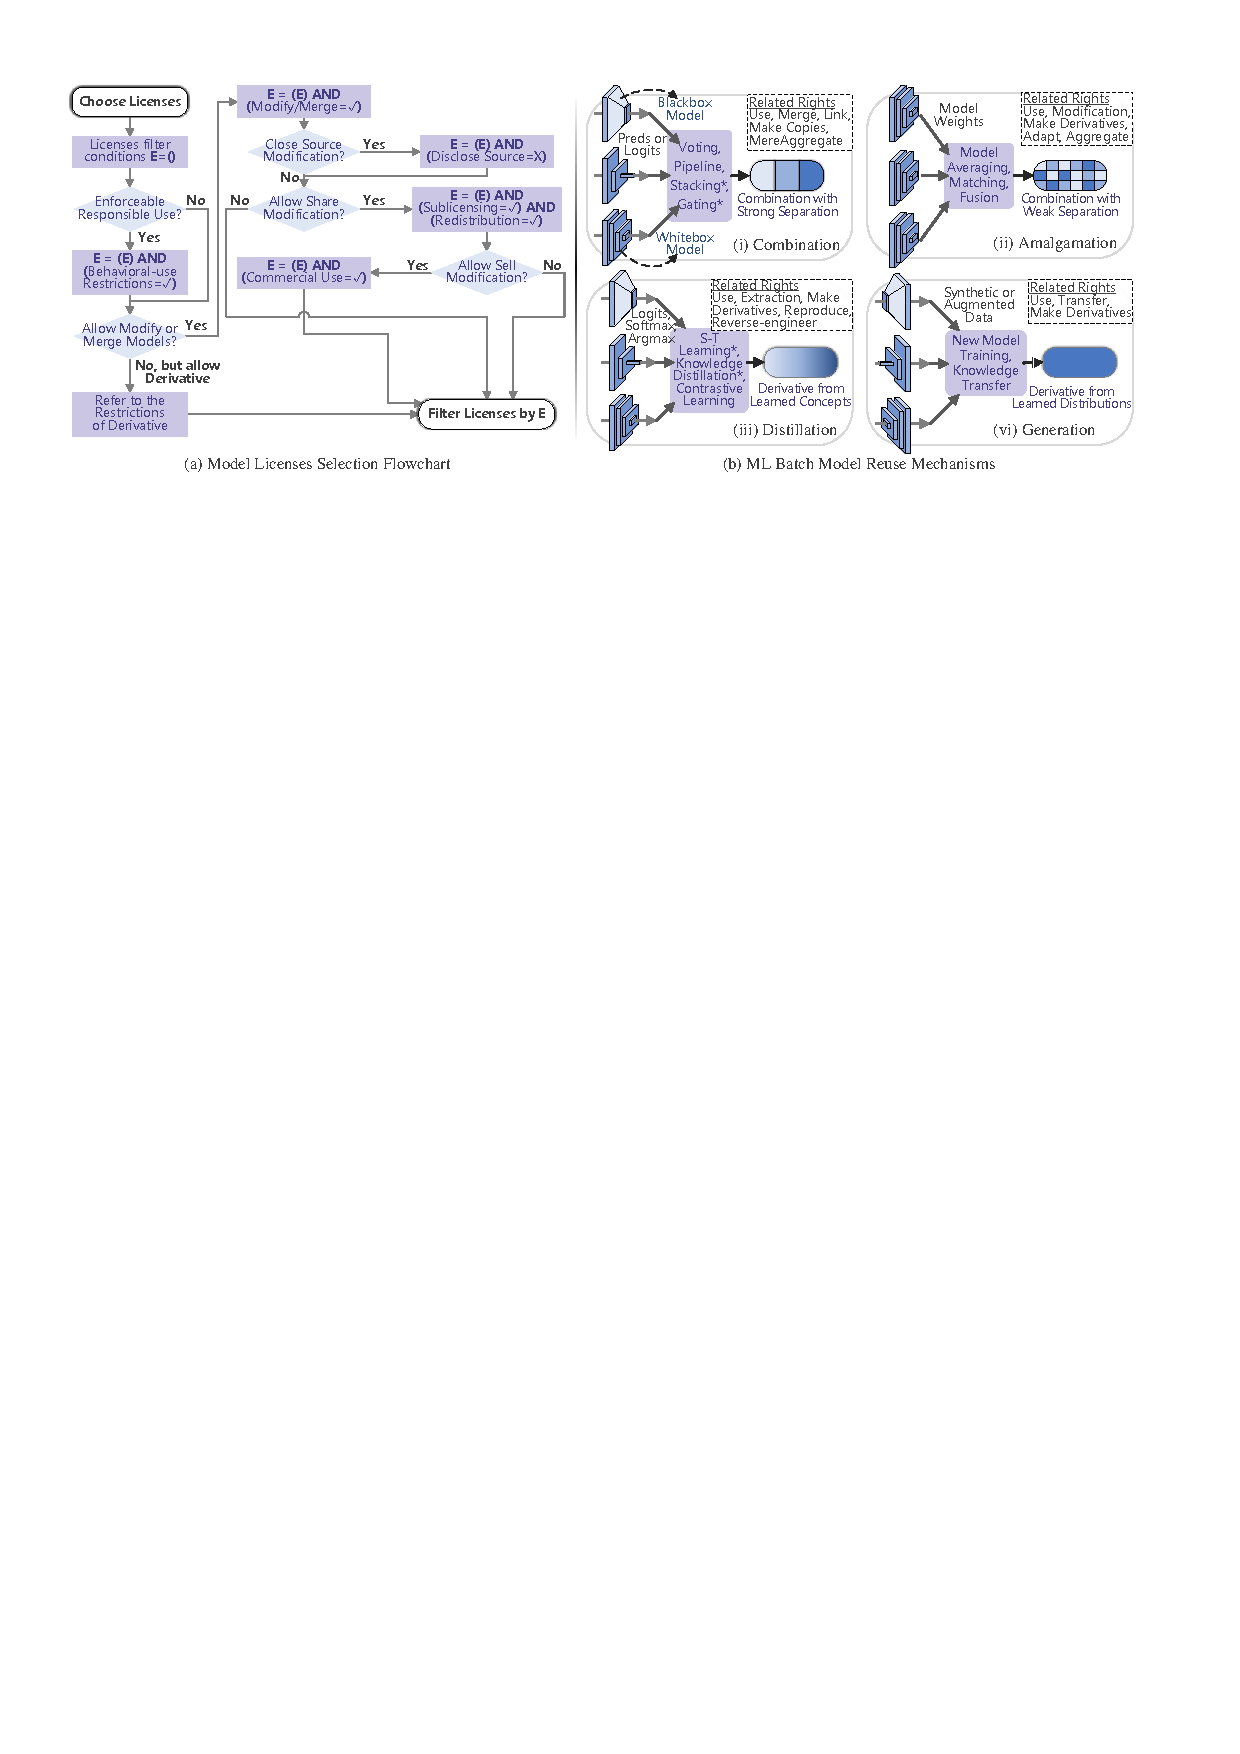
\includegraphics[width=\linewidth]{fig/flowchart.pdf}
    \caption{(a) Flowchart for model licenses selection in the context of model query and model reusing. (b) Proposed taxonomy categorizing batch model reuse mechanisms based on the reused results.}
    \label{fig:flowchart}
\end{figure*}

\subsection{Combination}
\label{sec:combination}
Combination~\cite{zhou2012ensemble} is a straightforward way to reuse batch of models (base learners), in which multiple models jointly contribute to the output by combination strategies such as averaging, voting, stacking~\cite{jacobs1991adaptive, wolpert1992stacked}.
For regression estimates, averaging can improve the generalization by taking the mean of the outputs of all weak learners in a population. Additionally, the outputs of each learner can be weighted by extra parameters~\cite{perrone1995networks}, which can be determined by stacking estimators~\cite{wolpert1992stacked}, Bayesian approach~\cite{clarke2003comparing} or backpropagation of gating networks~\cite{jacobs1991adaptive}. 
% Bayesian Model Averaging (BMA) -> Stacking with probabilities
Voting is a workaround strategy for classification tasks and also applicable for stacking and gating.
Both stacking and gating rely on a holdout or validation dataset for calculating extra parameters, marked as * in Fig.~\ref{fig:flowchart}(b). 
The difference is that gating can adapt the weights of each model's estimation based on the inputs, providing better generalizability performance of the combined model.

There are many advantages of combination mechanisms from the perspective of FL.
First, the input spaces of base models can be unaligned, which is ideal for the scenario of vertical FL~\cite{wu2022practical} where each client may have inconsistent features in their data.
Secondly, especially for query-based FL, it can simultaneously support multiple types and heterogeneous models, which means that it does not rely on any prior assumptions of the models, such as whether they are DNNs or decision trees, released with raw weights (whitebox) or binary forms (blackbox).
Thirdly, the tasks of models can be different if we pipeline the base models end-to-end, which is usually overlooked as a combination mechanism of models. 
Pipelining can fully leverage the transferability of models to solve previously unexplored ML problems.
% 举例说明 pipeline
For instance, Gao \textit{et al.}~\cite{gao2022precise} proposed a zero-shot dense retrieval system named HyDE by pipelining a natural language generation (NLG) model~\cite{ouyang2022training} and a natural language understanding (NLU) model~\cite{izacard2022unsupervised}.
The generated content, which may lack factual grounding, from the NLG model is used as query embeddings to facilitate real document retrieval by the NLU model.
Similarly, through query-based FL, we can query a vicarious NLG model for a novel scenario, such as ProGen~\cite{madani2023large} for protein sequences generation, and quickly adapt this system to proteomics.
Not limited to that, we can query a batch of NLG models by a well-chosen filter condition and then combine models through averaging or gating to significantly expand the exploration space for knowledge discovery.

Lastly, the combinated models have strong separation from each other, meaning that we can add or remove a batch of models without significant changes to the remaining ones.
Meanwhile, combination mechanisms do not rely on the transparency of models and support blackbox sharing. 
Thus, the base model can establish loose connections with other models only through run scripts, providing revocability of such combination and circumvention of the restrictions of licenses.
On the other hand, instead of being treated as a challenge for FL~\cite{ma2022state}, the statistical heterogeneity and model heterogeneity nature of these crowdsourced models can actually enrich population diversity, which is crucial for creating a good ensemble~\cite{maclin1995combining, opitz1995generating}. 

However, the storage consumption of combined models increases linearly with the number of base learners, which can strain the communication resources of a collaborative model training network. 
As a result, alternative approaches involve amalgamating or merging multiple models to create a new consensus model. 
In the following, we provide a summary of these methods.

\subsection{Amalgamation}
\label{sec:amalgamation}
Amalgamation involves combining models through model parameters granularity operations, such as median~\cite{blanchard2017machine, pillutla2022robust} and coordinate-wise averaging with consideration of heterogeneity~\cite{mcmahan2017communication, li2018federated}, security~\cite{sun2019can}, scalability~\cite{reisizadeh2020fedpaq}, matching~\cite{wang2020federated, yu2021fed2}, specificality~\cite{gudur2020resource}, generalizability~\cite{qu2022generalized}, resulting in a combination with weak separation.
This reusing approach is widely used in FL works and is often referred to as "aggregation" procedures for local models.
%Here, we avoid using the term "aggregation" to distinguish it from "combination" given the latter is often used interchangeably with "combination" in software licenses (e.g. Artistic, GPL).
However, in order to avoid confusion with the term "combination," which is frequently used interchangeably with "aggregation" in software licenses (e.g., Artistic, GPL), we opt to use the term "amalgamation" instead.

FedAvg~\cite{mcmahan2017communication} is the most popular model averaging method in FL with many follow-up works. 
For instance, Sun \textit{et al.}~\cite{sun2019can} proposed applying norm thresholding of local model updates to defend against backdoor attacks.
Similarly, Blanchard \textit{et al.}~\cite{blanchard2017machine} proposed using more robust median-based amalgamation for resilience against Byzantine behavior.
Consider the ordering of parameters, Wang \textit{et al.}~\cite{wang2020federated} match and average the NNs parameters layer-wise across clients, based on their similarities.
Yu \textit{et al.}~\cite{yu2021fed2} further attribute the misalignment in FL models to the non-IID training data, and propose allocating an independent structure for each class and updating models through a feature paired averaging strategy.

While amalgamation mechanisms can achieve a balance between model performance and resource efficiency by maintaining only one global model, they often rely on multiple rounds of communication to converge, which is not applicable in a query-based FL scenario.
Therefore, instead of trying to directly concatenate multiple sources of models while dealing with intricate parameter mismatch, transferring the latent knowledge learned by local models to a new model is a good alternative (i.e. Federated Distillation~\cite{jeong2018communication, jin2023feddyn}).

Another direction of model amalgamation is leveraging Bayesian nonparametrics to learn the shared global latent structures among local models~\cite{yurochkin2019bayesian, yurochkin2019statistical, lam2021model}. 
These methods, known as Model Fusion, can identify distributions of neural components across local models and only fuse the components with the same distribution, which can be regarded as a model compression between FedAvg (coordinate-wise averaging) and combination (w/o averaging).
However, the model fusion strategies rely on multiple communication rounds to boost the fusion efficiency, and the model performance of one-shot fusion is even worse than that of Ensemble.
Most recently, Su \textit{et al.}~\cite{su2023one}, inspired by null-space in continual learning~\cite{wang2021training, kong2022balancing}, propose MA-Echo which leverages layer-wise projection matrices to preserve the original loss of local models after amalgamation.
Their results present a moderate improvement in one-shot setting compared to FedAvg and ensemble.

Unfortunately, this improvement is not consistently observed in multiple-round experiments.
Meanwhile, to tackle the issue of catastrophic forgetting, FedPR~\cite{feng2023learning} follows similar ideas to facilitate the server's learning of visual prompts from clients for MRI reconstruction applications, but the improvement is limited even in multi-round setting. %compared to FedAvg

It is worth noting that our taxonomy is based on the form of the resulting model, which may not be entirely consistent with the terminology used in the technical perspective.
For example, Bayes Model Averaging (BMA)~\cite{clarke2003comparing} estimates posterior probabilities of each model given the observed data, which results in a separable weighted model. 
Therefore, it should be classified as Combination instead of Amalgamation like FedAvg.
This novel taxonomy method is useful for analyzing compatibility with licenses. 
For example, the coordinate-wise operations or the fusion of model parameters generate fine-grained combinations of models that are almost irreversible, which corresponds to clauses such as adapt, modify, dynamic link, and etc., in software licenses.

\begin{table*}[t]
  \centering
  \scriptsize
  \caption{Summary of privacy-preserving \textbf{Distillation} works in the field of FL. Some works are listed multiple times because they contain multiple KD procedures with different strategies. Works with naming conflicts are distinguished by subscript.}
  \label{tab:distillation}
  \begin{tabular}{|ll|p{12cm}|}
    \hline
    \multicolumn{2}{|l|}{Strategies} & FL Studies \\ \hline
    \multicolumn{1}{|l|}{\multirow{2}{*}{KD@Server}} & w/ Validation Set & FedED~\cite{sui2020feded} \\ \cline{2-3} 
    \multicolumn{1}{|l|}{} & w/ Unlabeled Data & FedDF~\cite{lin2020ensemble}, One-shot FL~\cite{guha2018one}, FedBE~\cite{chen2020fedbe}, PerAda~\cite{xie2023perada}, FedET~\cite{cho2022heterogeneous} \\ \hline
    \multicolumn{1}{|p{1.6cm}|}{\multirow{4}{*}{\shortstack{KD@Client \\ w/ Local Data}}} & from Global Model & FedFusion~\cite{yao2019towards}, FedKD\textsubscript{2}~\cite{wu2022communication}, MOON~\cite{li2021model}, FedNTD~\cite{lee2022preservation},  FedMLB~\cite{kim2022multi}, FedCAD~\cite{he2022class}, FedAlign\textsubscript{1}~\cite{mendieta2022local}, FedAlign\textsubscript{2}~\cite{zhang2023navigating}  \\ \cline{2-3} 
    \multicolumn{1}{|l|}{} & from Other Clients' Model  & FedMatch~\cite{jeong2020federated}, CCL~\cite{aketi2024cross}, FedProto\textsubscript{1}~\cite{michieli2021prototype}, FedProto\textsubscript{2}~\cite{tan2022fedproto} \\ \cline{2-3} 
    \multicolumn{1}{|l|}{} & from Self Model & FedFusion~\cite{yao2019towards}, FedDistill~\cite{jiang2020federated}, FedKD\textsubscript{2}~\cite{wu2022communication}, MOON~\cite{li2021model}, FCCL~\cite{huang2022learn}, pFedSD~\cite{jin2022personalized}, RSCFed~\cite{liang2022rscfed}, CCL~\cite{aketi2024cross} \\ \hline
    \multicolumn{2}{|l|}{KD w/ Public Unlabeled Datasets} & FedKT~\cite{li2021practical}, FedMD~\cite{li2019fedmd}, FedAD~\cite{gong2021ensemble}, FedMD-NFDP~\cite{sun2020federated}, FCCL~\cite{huang2022learn}, FedAUX~\cite{sattler2021fedaux}, RHFL~\cite{fang2022robust}, FedKD\textsubscript{1}~\cite{gong2022preserving}, Cronus~\cite{chang2021cronus}, KT-pFL~\cite{zhang2021parameterized}, DS-FL~\cite{itahara2021distillation} \\ \hline
    \multicolumn{2}{|l|}{KD w/ Generated Data (DFKD)} & DENSE~\cite{zhang2022dense}, FedCAVE-KD~\cite{heinbaugh2023data}, FedGen~\cite{zhu2021data},
    FedFTG~\cite{zhang2022fine} \\ \hline 
    \multicolumn{2}{|l|}{KD w/ Differential Privacy} & FedKC~\cite{wang2022fedkc}, FedSSL~\cite{fan2022private}  \\ \hline
    \end{tabular}
\end{table*}

\subsection{Distillation}
\label{sec:distillation}
Distillation was initially proposed by Hinton \textit{et al.}~\cite{hinton2015distilling} to transfer knowledge from a batch of independently trained neural network models (Specialists) to create a new Generalist model.
Their motivation was to explore the parallelization of training of specialists and improve the efficiency of distributed NNs modeling\cite{dean2012large}.
Each specialist only learns fine-grained distinctions of a subset of classes, which is very similar to the non-IID setting in FL~\cite{liqb2022federated}.
By using Knowledge Distillation (KD), we can also compress wide and deep teacher networks into lightweight student networks~\cite{romero2015fitnets}, which is promising for addressing system heterogeneity in cross-device FL~\cite{lim2020federated}.
Therefore, it is natural to extend the KD technologies to FL filed~\cite{wu2022communication}.
%~\cite{jiang2020federated, li2021practical, li2019fedmd, wu2022communication, chen2020fedbe, lin2020ensemble, gong2021ensemble, sun2020federated}.
Many recent FL works~\cite{aketi2024cross, luo2022fediris, tan2022fedproto}
%li2019fedmd, gong2021ensemble, sun2020federated, huang2022learn, fang2022robust, gong2022preserving, luo2022fediris, sui2020feded, chang2021cronus, he2020group, zhang2021parameterized, itahara2021distillation, aketi2024cross, michieli2021prototype, tan2022fedproto}
solely leverage KD without following the model averaging paradigm of FedAvg, we leave this discussion for later. %TODO

Despite directly retraining a Generalist model through KD, an alternative approach is to construct an ensemble of knowledge.
For example, Furlanello \textit{et al.}~\cite{furlanello2018born} consecutively generate student models with the guidance of knowledge distilled from earlier generations and find that the ensemble of multiple generations of internal models achieves state-of-the-art performance.
Dvornik \textit{et al.}~\cite{dvornik2019diversity} leverage the distilled knowledge from each learner to encourage cooperation and prediction diversity within the population, which leads to better ensemble results.
In the context of FL, the \emph{main advantage} of distillation is the decoupling between KD and knowledge learning. 
This allows us to split the model architecture for the purpose of system heterogeneity and efficiency~\cite{vepakomma2019split, thapa2022splitfed}.
Moreover, the well-learned knowledge from clients only needs to be communicated once~\cite{gong2021ensemble, gong2022preserving}, while the server can perform multiple epochs of local training to complete the transfer.

The drawback of KD is that it is data-dependent and the shared knowledge may be extracted from local sensitive data, which exposes a new attack surface for potential model inversion attacks~\cite{kim2020multiple, fredrikson2015model}.
To mitigate this issue, some efforts~\cite{wang2022fedkc, fan2022private} have been made to add differential privacy noise~\cite{dwork2006differential} to the shared content.

In general, there are three mechanisms for avoiding the sharing of sensitive knowledge.
First, push the KD procedure to the server-side, where the knowledge of local models is transferred to the global model through a validation set~\cite{sui2020feded} or unlabeled dataset~\cite{lin2020ensemble, guha2018one, chen2020fedbe, xie2023perada, cho2022heterogeneous} held by the server.
Second, we can keep the KD procedure at the client-side, allowing the knowledge of the global model~\cite{yao2019towards, wu2022communication,li2021model, lee2022preservation, mendieta2022local, kim2022multi, he2022class, zhang2023navigating}, other clients' models~\cite{jeong2020federated, aketi2024cross, michieli2021prototype, tan2022fedproto} or self-model~\cite{yao2019towards, jiang2020federated, wu2022communication, li2021model, huang2022learn, jin2022personalized, liang2022rscfed} to be transferred based on the local training data.
In the above two strategies, only model parameters are exchanged in the training network, which means they can provide the same level of privacy protection as traditional FL.

%The last mechanism assumes that a public unlabeled dataset is accessible to both the server and clients for KD~\cite{li2021practical, li2019fedmd, gong2021ensemble, sun2020federated, huang2022learn, sattler2021fedaux, fang2022robust, gong2022preserving, chang2021cronus, zhang2021parameterized, itahara2021distillation}.
The last mechanism is to assume that a public unlabeled dataset, which is non-sensitive, is accessible by both the server and clients for KD~\cite{li2021practical, li2019fedmd, gong2021ensemble, sun2020federated, huang2022learn, sattler2021fedaux, fang2022robust, gong2022preserving, chang2021cronus, zhang2021parameterized, itahara2021distillation}.
Sharing these extracted contents will not raise any privacy concerns, and only minimal communication is generated during KD for the purpose of aligning sample IDs.
In cases where such public datasets are not available on the server, a recent approach known as Data-Free Knowledge Distillation (DFKD)~\cite{lopes2017data} regenerates batches of data based on layer activation statistics or spectrum coefficients collected during training phase. 
Then, this synthetic data is used for distillation.
DENSE~\cite{zhang2022dense} is the first attempt to extend DFKD to FL. It leverages the ensemble of local models to guide the training of a data generator on the server, and the generated data is then used to distill the knowledge from local models to the global model.
FedCAVE-KD~\cite{heinbaugh2023data} leverages locally trained conditional autoencoders (CVAEs)~\cite{kingma2014auto} to generate samples based on the data distribution of clients. 
These CVAEs are sent to server used to construct a global generator via KD, which will later provide synthetic training data for the global discriminator.

It is worth noting that in the query-based FL setting, direct access to the original data is not available, thus the second mechanism mentioned earlier cannot be directly applied.
A circumvention method is to train a generator following the inspiration of DFKD. 
Fortunately, this is praticable if the workflow and history information of modeling are tracked and queryable, as we advocated in \S\ref{sec:how2query}.
Recalling that, as shown in Fig.~\ref{fig:flowchart}(b), Generation is the last category in our taxonomy.
Actually, such a hybrid model reuse strategy is quite common in FL. 
For example, the previously mentioned DENSE~\cite{zhang2022dense} incorporates three model reuse mechanisms: Combination (creating an ensemble), Generation (generating synthetic data), and Distillation.
Therefore, our taxonomy can cover traditional FL works, such as FedAvg and MOON~\cite{li2021model}, as well as the broad sense FL, including Federated Distillation~\cite{jeong2018communication, jin2023feddyn} and Ensemble Learning~\cite{shi2023fed, wang2023data}.
We provide a comparison of these hybrid works in \S\ref{sec:hybrid}. 
The summarization of above privacy-perserving KD works is given in TABLE.~\ref{tab:distillation}.

% the model trained in one specific domain cannot well generalize to other domains
% KD 是用于加速网络训练,属于分布式机器学习范畴

% KD 的优点:不需要相同的模型结构,缺点:依赖数据, Data-dependent KD, extracted soft labels 参考:Related work of DYNAFED: Tackling Client Data Heterogeneity with Global Dynamics 

\subsection{Generation}
\label{sec:generation}
Generation is designed to generate synthetic samples that resemble the original data distribution by building a probabilistic model~\cite{geyer1992practical} or deep learning model~\cite{kingma2014auto, goodfellow2020generative, cao2022survey} that can capture the underlying distribution pattern and latent structure of original data.
Generally speaking, generation techniques can be classified into three categories: data-level, probabilistic, and representation-based approaches.
Data-level approaches involve sample granularity operations such as interpolation~\cite{chawla2002smote, zhangmixup} and augmentation~\cite{wong2016understanding} to generate synthetic features based on the original feature space of data and share.
Even though these methods are training-free and easy to implement, they cannot be directly applied to the FL setting due to privacy concerns.
Recent proposed FedMix~\cite{yoon2021fedmix} aims to alleviate the negative effect of non-IID data by using \textit{mixup}~\cite{zhangmixup}, where the average of local data is linearly interpolated with the training data to generate augmented samples.
However, the potential risk of data leakage when sharing the mixup data is not comprehensively evaluated in the original work.

Probabilistic approachs aim to estimate the real data distribution using probabilistic method.
For example, Markov Chain Monte Carlo (MCMC)~\cite{geyer1992practical} methods construct a Markov Chain that converges to the desired target distribution by iteratively proposing new states based on the current state of the chain and acceptance probabilities.
Gaussian Mixture Models (GMM) assumes the data is generated from a mixture of Gaussian distributions and can generate new samples by sampling from the learned distributions.
To generate the high-dimensional structured data, representation-based approaches try to reconstruct the data from laten feature space.
For instance, Variational Autoencoders (VAEs)~\cite{kingma2014auto} learn the distribution of the latent representation space given the observed data and then use a decoder network to reconstruct data based on sampled latent representations.
Generative Adversarial Networks (GANs)~\cite{goodfellow2020generative} train a generator network to produce samples that resemble realistic data by optimizing an adversarial objective against a discriminator network.

Compared to the other model reuse mechanisms, generation has three unique advantages.
The first advantage is visualization and verification. Unlike the extracted knowledge in distillation, the quality of generated content can be visualized and validated by humans. 
This capability aids in assessing the contributions made by participants in terms of generating valuable content.
Second, the flexibility of generation methods allow us to generate data with any desired amount or class, which enables more effective handling of imbalanced~\cite{chawla2002smote} and non-IID~\cite{zhang2022fine} data.
The third advantage is multi-format sharing. Participants have the freedom to choose the form of their contributions. For example, they can upload the learned generative models in source code (e.g., Stable Diffusion~\cite{rombach2022high}, GPT-2~\cite{radford2019language}) or binary form, upload synthetic data, or provide model inference APIs like ChatGPT.
This sharing policy can greatly empower the model community in open FL platforms, fostering collaboration and knowledge sharing.

Given the aforementioned advantages, generation methods have been extensively studied in the field of FL. 
As summaried in TABLE.~\ref{tab:generation}, these works can be classified into two main categories: generation for training~\cite{zhang2021subgraph, cheng2023gfl, hao2021towards, cha2019federated, yu2023turning, heinbaugh2023data, yang2023exploring, liu2021feddg, pi2023dynafed, liz2022federated, diao2022semifl}, generation for KD~\cite{zhang2022dense, chen2020fedbe, zhu2021data, zhang2022fine, jeong2018communication, jin2023feddyn, heinbaugh2023data, zhang2022fedzkt, fan2022private}, and serving three purposes: enriching the training set~\cite{zhang2022dense, chen2020fedbe, zhang2021subgraph, cheng2023gfl, cha2019federated, jin2023feddyn, zhang2022fedzkt}, improving generalization ability~\cite{zhu2021data, zhang2022fine, hao2021towards, jeong2018communication, yu2023turning, heinbaugh2023data, liu2021feddg, pi2023dynafed, liz2022federated}, and enabling semi-supervised learning~\cite{yang2023exploring, diao2022semifl, fan2022private}.
As an example of generation for training, FedSage+~\cite{zhang2021subgraph} trains a missing neighbors generator to mend the links between cross-subgraph nodes, thereby increasing the connectivity of local data and benefiting from this collaboration across clients.
Previously mentioned FedCAVE-KD~\cite{heinbaugh2023data} is an example of generation for KD, where locally trained CVAEs and local label distributions are uploaded to the server for DFKD, ensuring privacy while also enhancing generalization of global model.
Another example is FedGen~\cite{zhu2021data}, where the generator is maintained by the server and sent to clients in each round.
The generator has knowledge about the global view of the data distribution, which is used to KD into the local models, thereby enhancing their generalizability.
The last application of generation is in semi-supervised learning, which is a common real-world scenario where the client data is unlabeled.
For example, FedDISC~\cite{yang2023exploring} leverages the average and cluster centroids of hidden representations across pseudo-labels as input to a pre-trained diffusion model, aiming to generate high-quality samples for training.

In fact, the three purposes of generation correspond to three types of data heterogeneity in FL~\cite{liqb2022federated}: Quantity Skew, Label Distribution Skew (non-IID), and Missing Labels, which are challenging to address with traditional model amalgamation methods.
The hybrid model reusing strategies, which leverage each other's strengths, have become a common paradigm in recent FL studies~\cite{cheng2023gfl, xie2023perada, yu2023turning, jin2023feddyn, heinbaugh2023data, yang2023exploring, zhang2023navigating}.
Therefore, in the next section, we will summarize the popular hybrid model reusing studies in FL and then filter the studies that are suitable for query-based FL platforms.

\begin{table}[t]
  \centering
  \tiny
  \caption{Classification of \textbf{Generation} works in the field of FL. Some of the works are also listed in TABLE~\ref{tab:distillation} because they utilize hybrid model reuse mechanisms.}
  \label{tab:generation}

  \begin{tabular}{|l|p{2.1cm}|p{2.3cm}|p{1.45cm}|}
    \hline
    & Enriching Training Set & Improving Generalization  & Enabling Semi-supervised Learning  \\ \hline
   
    \multicolumn{1}{|l|}{For Training} & FedSage+~\cite{zhang2021subgraph}, GFL~\cite{cheng2023gfl}, \newline FRD~\cite{cha2019federated} & Fed-ZDA~\cite{hao2021towards}, FedDG~\cite{liu2021feddg}, FOSTER~\cite{yu2023turning}, DynaFed~\cite{pi2023dynafed}, SDA-FL~\cite{liz2022federated}, FedMix~\cite{yoon2021fedmix}, \newline FedCAVE-Ens~\cite{heinbaugh2023data} & FedDISC~\cite{yang2023exploring}, \newline SemiFL~\cite{diao2022semifl}  \\ \hline

    \multicolumn{1}{|l|}{For KD} & DENSE~\cite{zhang2022dense}, FedBE~\cite{chen2020fedbe}, \newline FedDyn~\cite{jin2023feddyn}, FedZKT~\cite{zhang2022fedzkt} & FedGen~\cite{zhu2021data}, FedFTG~\cite{zhang2022fine}, FD+FAug~\cite{jeong2018communication}, FedCAVE-KD~\cite{heinbaugh2023data} & FedSSL~\cite{fan2022private} \\ \hline
  \end{tabular}
\end{table}

%The third advantage is free-sharing. As mentioned in Section~\ref{sec:generated content}, many deep generative models, such as Stable Diffusion~\cite{rombach2022high} and ChatGPT, do not claim ownership rights over the generated content. Furthermore, most OSS licenses do not have defined terms for computer-generated content. Therefore, it is legally permissible to freely reuse synthetic data.

% 三种方法:1,data level(如SMOTE, augmentation)2, 概率模型(MCMC, 自回归模型) 3,sample from latent representation(GAN,CVAE)
% 优点:1,生成的内容质量容易被校验(相比KD)2,可以掌控生成物的数量 3,弱连接(甚至不需要保留模型)
% 生成物的用法:1,重新训练 2,KD 3,提升模型鲁棒性和平衡性

%也可以是基于数据的生成

\subsection{Hybrid Model Reusing and Model Licenses}
\label{sec:hybrid}
Following the taxonomy we introduced in \S\ref{sec:taxonomy}, it can be observed that almost all FL studies can be regarded as a permutation of four model reuse mechanisms: Combination, Amalgamation, Distillation, and Generation.
To enhance our understanding of current model reusing studies and identify methods applicable for constructing an open FL platform, we provide a comprehensive summary in TABLE~\ref{tab:flreuse}.
We employ different colors and fonts in TABLE~\ref{tab:flreuse} to emphasize the distinctions among studies, while certain processes have been omitted without ambiguity.
In addition, we have listed the main goals of each study, and only those with explicit designs, experiments, or proof are counted.
Please refer to the table caption for the explanation of our denotations.
As an example, the process of RSCFed~\cite{liang2022rscfed} involves the following steps: 
\ding{172} KD, the knowledge is extracted as the softmax values from the self model based on local private data (ref. TABLE.~\ref{tab:distillation}) and performed at the client-side;
\ding{173} Model exponential moving averaging performed at the client-side;
\ding{174} Simple Model Averaging performed two times at the server-side.
These processes are repeated across multiple communication rounds until completion.
In this way, we can categorize these works and make intuitive comparisons between them\textsuperscript{\ddag{IV-A}}.
%Due to page limits, we leave the detailed analysis in Appendix~IV.A.

Through disassembling hybrid model reusing into the four model reuse mechanisms, we can further analyze the corresponding clauses in model licenses perspective for FL studies.
Then we can easily identify the applicable clauses for different model reusing mechanisms\textsuperscript{\ddag{IV-A}}.
%We present the detailed methodology in Appendix~IV.B.

\begin{table*}[htp]
  \centering
  \scriptsize
  \caption{Comparative analysis of FL studies categorized by our taxonomy for batch model reuse mechanisms.
  Studies \textcolor{red}{applicable} and \textcolor{orange}{conditional applicable} to query-based FL are marked with different colors;
  \textcolor{purple}{Purple} denotes operations completed on \textcolor{purple}{Server}, or knowledge distilled from \textcolor{purple}{Global or Consensus Model}; 
  \textcolor{blue}{Blue} denotes operations completed on \textcolor{blue}{Clients}, or knowledge distilled from \textcolor{blue}{Local, Personlized, or Generative Models}; 
  \textbf{Knowledge} or \textbf{Generated Content} based on \textbf{Public, Proxy or Generated} data, and \textit{Knowledge} or \textit{Generated Content} based on \textit{Local, Private or Sensitive} data;
  [~]*1: one round of communication (aka one-shot), [~]*N: multiple rounds of communication, processes ahead ...[~] are performed only once (i.e. preprocessing), processes inside [...] are main functional part; Slash "/": model training based on \textit{private} data, Comma ",": model training based on \textbf{non-sensitive} data; Goals of works: \textbf{E}fficiency \textbf{H}eterogeneity \textbf{P}rivacy.}
  %\vspace{-6mm}
  \label{tab:flreuse}
  %\setlength\arrayrulewidth{0.001pt}
  \begin{tabular}{|p{2.05cm}|p{1.36cm}|p{1.56cm}|p{4.35cm}|p{2.77cm}|p{1.5cm}|p{0.35cm}|}
    \hline
    \rowcolor[gray]{.8}
    \multicolumn{1}{|c|}{FL Studies} & \multicolumn{1}{c|}{\textbf{C}ombination} & \multicolumn{1}{c|}{\textbf{A}malgamation} & \multicolumn{1}{c|}{\textbf{D}istillation} & \multicolumn{1}{c|}{\textbf{G}eneration} & \multicolumn{1}{c|}{Process}& \multicolumn{1}{c|}{Goals} \\ \hline
    FedAvg~\cite{mcmahan2017communication} & n/a &  \textcolor{purple}{Model Avg}  & n/a & n/a & [\textcolor{blue}{/}\textcolor{purple}{A}]*N & EH   \\ \hline

    \rowcolor[gray]{.9}
    \textcolor{red}{FedAD}~\cite{gong2021ensemble} & n/a & n/a & \textcolor{purple}{KD} \textcolor{blue}{\textbf{Attention, Logits}}  & n/a & \textcolor{blue}{/}[\textcolor{purple}{D}]*1 & HP \\ \hline %CC
  
    \textcolor{red}{FedKD\textsubscript{1}}~\cite{gong2022preserving} & n/a & n/a & \textcolor{purple}{KD} \textcolor{blue}{\textbf{Weighted Logits}} & n/a &\textcolor{blue}{/}[\textcolor{purple}{D}]*1 & EHP \\ \hline %CC

    \rowcolor[gray]{.9}
    \textcolor{red}{FedED}~\cite{sui2020feded} & n/a & n/a & \textcolor{purple}{KD} \textcolor{blue}{\textbf{Logits Avg on Global Validation Data}} & n/a &[\textcolor{blue}{,}\textcolor{purple}{D}]*N & EHP \\ \hline %CC 

    FedIris~\cite{luo2022fediris} & n/a & n/a & \textcolor{blue}{KD \textit{Hidden}} & n/a &[\textcolor{blue}{D}]*N & H \\ \hline %CC

    \rowcolor[gray]{.9}
    FedProto~\cite{tan2022fedproto} & n/a & n/a & \textcolor{blue}{KD \textit{Per-Class Hidden Avg}} & n/a &[\textcolor{blue}{/D}]*N & EH \\ \hline %CC

    FedMD~\cite{li2019fedmd} & n/a & n/a & \textcolor{blue}{KD \textbf{Logits Avg}} & n/a &[\textcolor{blue}{D/}]*N & H \\ \hline %CC

    \rowcolor[gray]{.9}
    FedMD-NFDP~\cite{sun2020federated}& n/a & n/a & \textcolor{blue}{KD \textbf{Logits/Softmax/Argmax Avg}} & n/a & \textcolor{blue}{/}[\textcolor{blue}{D/}]*N & HP \\ \hline %CC

    DS-FL~\cite{itahara2021distillation}& n/a & n/a & \textcolor{blue}{KD \textbf{Entropy Reduced Logits Avg}} & n/a &[\textcolor{blue}{/D}]*N & EH \\ \hline %CC

    \rowcolor[gray]{.9}
    \textcolor{red}{RHFL}~\cite{fang2022robust} & n/a & n/a & \textcolor{blue}{KD \textbf{Weighted Logits}} & n/a & \textcolor{blue}{/}[\textcolor{blue}{D}]*N & EH \\ \hline

    KT-pFL~\cite{zhang2021parameterized} & n/a & n/a & \textcolor{blue}{KD \textbf{Learned Weighted Softmax}} & n/a &[\textcolor{blue}{/D}]*N & EH \\ \hline

    \rowcolor[gray]{.9}
    Cronus~\cite{chang2021cronus} & n/a & n/a & \textcolor{blue}{KD} \textcolor{blue}{\textbf{Robust Mean Estimation of Softmax}} & n/a & \textcolor{blue}{/}[\textcolor{blue}{/D}]*N & EHP \\ \hline
    
    FedDISC~\cite{yang2023exploring} & n/a & n/a & n/a & \textcolor{purple}{\textit{Synthetic Data}} &[\textcolor{purple}{G}]*1\textcolor{purple}{,} & EH \\ \hline

    \rowcolor[gray]{.9}
    FRD~\cite{cha2019federated} & n/a & n/a & n/a & \textcolor{purple}{\textit{Mixup Data}} &[\textcolor{purple}{G}]*1\textcolor{purple}{,} & E \\ \hline

    \textcolor{red}{One-Shot FL}~\cite{guha2018one} & \textcolor{purple}{Output Avg} & n/a & \textcolor{purple}{KD} \textcolor{blue}{\textbf{Softmax}} & n/a & \textcolor{blue}{/}[\textcolor{purple}{CD}]*1 & EP \\ \hline %CC

    \rowcolor[gray]{.9}
    FedDF~\cite{lin2020ensemble} & n/a & \textcolor{purple}{Model Avg} & \textcolor{purple}{KD}  \textcolor{blue}{\textbf{Logits Avg}} & n/a & [\textcolor{blue}{/}\textcolor{purple}{AD}]*N & HP \\ \hline %CC

    PerAda~\cite{xie2023perada} & n/a & \textcolor{purple}{Adapter Avg} & \textcolor{purple}{KD} \textcolor{blue}{\textbf{Logits Avg}} & n/a & [\textcolor{blue}{//}\textcolor{purple}{AD}]*N & EHP \\ \hline

    \rowcolor[gray]{.9}
    FedFiMa~\cite{che2022federated} & n/a & \textcolor{purple}{Rep. Layer Avg} & \textcolor{blue}{KD} \textcolor{blue}{\textbf{Hidden Avg}} & n/a & [\textcolor{blue}{/}\textcolor{purple}{A}\textcolor{blue}{D}]*N & EH \\ \hline

    FedFusion~\cite{yao2019towards} & n/a & \textcolor{purple}{Model Avg} & \textcolor{blue}{KD} \textcolor{blue}{\textit{Hidden}}, \textcolor{purple}{\textit{Hidden}} & n/a & [\textcolor{blue}{D}\textcolor{purple}{A}]*N & E \\ \hline %CC

    \rowcolor[gray]{.9}
    FedNTD~\cite{lee2022preservation} & n/a & \textcolor{purple}{Model Avg} & \textcolor{blue}{KD} \textcolor{purple}{\textit{Not-True Classes Softmax}} & n/a & [\textcolor{blue}{D}\textcolor{purple}{A}]*N & H \\ \hline %CC

    FedKC~\cite{wang2022fedkc} & n/a & \textcolor{purple}{Model Avg} & \textcolor{blue}{KD} \textcolor{blue}{\textit{Clustered Hidden Avg}} & n/a & [\textcolor{blue}{D}\textcolor{purple}{A}]*N & HP \\ \hline %CC

    \rowcolor[gray]{.9}
    FedDistill~\cite{jiang2020federated} & n/a & \textcolor{purple}{Model Avg} & \textcolor{blue}{KD \textit{Softmax of Latest Local Model}} & n/a &[\textcolor{blue}{/D}\textcolor{purple}{A}]*N & H \\ \hline %CC

    pFedSD~\cite{jin2022personalized} & n/a & \textcolor{purple}{Model Avg} & \textcolor{blue}{KD \textit{Softmax of Pervious Local Model}} & n/a &[\textcolor{blue}{/D}\textcolor{purple}{A}]*N & H \\ \hline

    \rowcolor[gray]{.9}
    FedMLB~\cite{kim2022multi} & n/a & \textcolor{purple}{Model Avg} &\textcolor{blue}{KD} \textcolor{purple}{\textit{Softmax, Scaled Softmax}} & n/a & [\textcolor{blue}{/D}\textcolor{purple}{A}]*N & EH \\ \hline %CC

    FedAlign\textsubscript{1}~\cite{mendieta2022local} & n/a &\textcolor{purple}{Model Avg}&\textcolor{blue}{KD}  \textcolor{purple}{\textit{Lipschitz Constants}}~\cite{shang2021lipschitz} & n/a & [\textcolor{blue}{/D}\textcolor{purple}{A}]*N & EH \\ \hline %CC
    
    \rowcolor[gray]{.9}
    MOON~\cite{li2021model} & n/a & \textcolor{purple}{Model Avg} & \textcolor{blue}{Contrastive Learning} \textcolor{purple}{\textit{Hidden}}, \textcolor{blue}{\textit{Hidden}} & n/a &[\textcolor{blue}{/D}\textcolor{purple}{A}]*N & EH \\ \hline %CC

    FedCAD~\cite{he2022class} & n/a & \textcolor{purple}{Model Avg} & \textcolor{blue}{KD} \textcolor{purple}{\textit{Class-Wise Softmax}} & n/a & [\textcolor{blue}{/D}\textcolor{purple}{A}]*N & H \\ \hline %CC

    \rowcolor[gray]{.9}
    FedGKT~\cite{he2020group} & n/a & n/a & \textcolor{blue}{KD} \textcolor{purple}{\textit{Logits}} \textcolor{purple}{KD} \textcolor{blue}{\textit{Logits, Hidden, Argmax}} & n/a & [\textcolor{blue}{/D}\textcolor{purple}{/D}]*N & EH \\ \hline

    FCCL~\cite{huang2022learn} & n/a & n/a & \textcolor{purple}{Contrastive Learning} \textcolor{blue}{\textbf{Logits Avg}} \newline \textcolor{blue}{Continual Learning} \textcolor{blue}{\textit{Logits}} & n/a & [\textcolor{purple}{D}\textcolor{blue}{/D}]*N & H \\ \hline %CC

    \rowcolor[gray]{.9}
    \textcolor{orange}{GFL}~\cite{cheng2023gfl} & n/a & \textcolor{purple}{Model Avg} & n/a & \textcolor{blue}{\textbf{Synthetic Data}} & \textcolor{blue}{/G}[\textcolor{blue}{,}\textcolor{purple}{A,}]*N & HP \\ \hline

    FOSTER~\cite{yu2023turning} & n/a & \textcolor{purple}{Model Avg} & n/a & \textcolor{blue}{\textbf{Synthetic Outliers}} & \textcolor{purple}{,}[\textcolor{blue}{G/}\textcolor{purple}{A}]*N & EH \\ \hline

    \rowcolor[gray]{.9}
    FedDG~\cite{liu2021feddg} & n/a & \textcolor{purple}{Model Avg} & n/a & \textcolor{blue}{\textbf{Interpolated Data}} & [\textcolor{blue}{G/}\textcolor{purple}{A}]*N & H \\ \hline  % 基于振幅的插值,可以认为不涉及隐私数据

    SemiFL~\cite{diao2022semifl} & n/a & \textcolor{purple}{Model Avg} & n/a & \textcolor{blue}{\textit{Augmented and Mixup Data}} & [\textcolor{purple}{,}\textcolor{blue}{G/}\textcolor{purple}{A}]*N & H \\ \hline 

    \rowcolor[gray]{.9}
    NeighGen~\cite{zhang2021subgraph} \newline FedSage~\cite{zhang2021subgraph} & & \textcolor{purple}{Gradient Avg}\newline\textcolor{purple}{Model Avg} & n/a &\textcolor{blue}{\textit{Synthetic Node}} & [\textcolor{blue}{G/}\textcolor{purple}{A}]*N \newline [\textcolor{blue}{/}\textcolor{purple}{A}]*N & H \\ \hline

    Fed-ZDAC~\cite{hao2021towards} & n/a & \textcolor{purple}{Model Avg} & n/a & \textcolor{blue}{\textbf{Zero-shot Synthetic Data}} & [\textcolor{blue}{G/}\textcolor{purple}{A}]*N & HP \\
    Fed-ZDAS~\cite{hao2021towards} & n/a & n/a & n/a & \textcolor{purple}{\textbf{Zero-shot Synthetic Data}} & [\textcolor{blue}{/}\textcolor{purple}{G,A}]*N & \\ \hline

    \rowcolor[gray]{.9}
    FedMix~\cite{yoon2021fedmix} & n/a & \textcolor{purple}{Model Avg} & n/a & \textcolor{purple}{\textit{Mixup Data}} \textcolor{blue}{\textit{Mixup Data}} & [\textcolor{purple}{GA\textcolor{blue}{,}}]*N\textcolor{blue}{G}\textcolor{blue}{,} & HP \\ \hline

    FedDyn~\cite{jin2023feddyn} & n/a & n/a & \textcolor{purple}{KD} \textcolor{blue}{\textit{Hidden, Logits Avg}} & \textcolor{blue}{\textbf{Synthetic Data}} & [\textcolor{blue}{/G}\textcolor{purple}{D}]*N & E \\ \hline

    \rowcolor[gray]{.9}
    FD+FAug~\cite{jeong2018communication} & n/a & n/a & \textcolor{blue}{KD} \textcolor{blue}{\textit{Per-Class Logits Avg}} & \textcolor{blue}{\textbf{Synthetic Data}} & [\textcolor{purple}{/}\textcolor{blue}{G}\textcolor{blue}{/D}]*N & EP \\ \hline

    \textcolor{red}{FedCAVE-Ens}~\cite{heinbaugh2023data} & \textcolor{purple}{Collection}  & n/a & n/a & \textcolor{purple}{\textbf{Synthetic Data}} & \textcolor{blue}{/}\textcolor{purple}{C}[\textcolor{purple}{G,}]*1 & H \\
    \textcolor{red}{FedCAVE-KD}~\cite{heinbaugh2023data} & n/a & n/a & \textcolor{purple}{KD} \textcolor{blue}{\textbf{Softmax}} & & \textcolor{blue}{/}\textcolor{purple}{C}[\textcolor{purple}{GDG,}]*1 & H \\ \hline

    \rowcolor[gray]{.9}
    Fed-ET~\cite{cho2022heterogeneous} & n/a & \textcolor{purple}{Rep. Layer Avg} \newline \textcolor{purple}{Model Avg} & \textcolor{purple}{KD} \textcolor{blue}{\textbf{Argmax, Weighted Logits}} & n/a & [\textcolor{blue}{/}\textcolor{purple}{ADA}]*N & EH \\ \hline

    \textcolor{orange}{FedBE}~\cite{chen2020fedbe} & n/a & \textcolor{purple}{Model Avg} & \textcolor{purple}{KD} \textcolor{blue}{\textbf{Softmax Avg}} & \textcolor{purple}{\textbf{Synthetic Model}} & [\textcolor{blue}{/}\textcolor{purple}{AGD}]*1 & H \\ \hline %CC

    \rowcolor[gray]{.9}
    DynaFed~\cite{pi2023dynafed} & n/a & \textcolor{purple}{Model Avg} & n/a & \textcolor{purple}{\textbf{Synthetic Data}} & [\textcolor{blue}{/}\textcolor{purple}{A}]*N\textcolor{purple}{G}[\textcolor{purple}{A,}]*N & EH \\ \hline

    \textcolor{orange}{FedAUX}~\cite{sattler2021fedaux} & n/a & \textcolor{purple}{Model Avg} & \textcolor{blue}{Contrastive Learning} \textcolor{purple}{\textbf{Hidden}, \textit{Hidden}} \newline \textcolor{purple}{KD} \textcolor{blue}{\textbf{Weighted Logits}} & n/a & \textcolor{purple}{,}\textcolor{blue}{D}[\textcolor{purple}{A\textcolor{blue}{/}D}]*N \newline \textcolor{purple}{,}\textcolor{blue}{D}[\textcolor{purple}{A\textcolor{blue}{/}D}]*1 & HP \\ \hline %CC
    
    \rowcolor[gray]{.9}
    FedKD\textsubscript{2}~\cite{wu2022communication} & n/a & \textcolor{purple}{Gradient Avg} & \textcolor{blue}{KD} \textcolor{purple}{\textit{Hidden, Attention, Logits}} \newline \textcolor{blue}{KD} \textcolor{blue}{\textit{Hidden, Attention, Logits}} & n/a & [\textcolor{blue}{/D}\textcolor{purple}{A}\textcolor{blue}{D}]*N & EH \\ \hline %CC

    FedGen~\cite{zhu2021data} & n/a & \textcolor{purple}{Model Avg} & \textcolor{purple}{KD} \textcolor{blue}{\textbf{Softmax}} \textcolor{purple}{KD} \textcolor{blue}{\textbf{Logits Avg}} & \textcolor{blue}{\textbf{Augmented Data}} & \textcolor{purple}{D}[\textcolor{blue}{/G,}\textcolor{purple}{AD}]*N & EHP \\ \hline %CC

    \rowcolor[gray]{.9}
    SDA-FL~\cite{liz2022federated} & n/a & \textcolor{purple}{Model Avg} & \textcolor{purple}{KD} \textcolor{blue}{\textbf{Argmax}} & \textcolor{blue}{\textbf{Synthetic Data}}\newline \textcolor{blue}{\textit{Augmented Data}} & \textcolor{blue}{/G}[\textcolor{blue}{G/}\textcolor{purple}{AD}]*N & HP \\ \hline

    FedKT~\cite{li2021practical} & \textcolor{blue}{Voting} \textcolor{purple}{Voting} & n/a & \textcolor{blue}{KD} \textcolor{blue}{\textbf{Argmax}} \textcolor{purple}{KD} \textcolor{blue}{\textbf{Argmax}} & n/a & [\textcolor{blue}{/CD}\textcolor{purple}{CD}]*1 & HP \\ \hline %CC %是否属于KD还是train取决于数据是否由其他模型生成的

    \rowcolor[gray]{.9}
    FedMatch~\cite{jeong2020federated} & \textcolor{blue}{Voting} & \textcolor{purple}{Model Avg} & \textcolor{blue}{KD} \textcolor{blue}{\textit{Argmax}} & n/a & [\textcolor{blue}{C/D}\textcolor{purple}{AA}]*N \newline [\textcolor{purple}{,}\textcolor{blue}{CD}\textcolor{purple}{A}]*N & EH \\ \hline %CC

    FedFTG~\cite{zhang2022fine} & n/a & \textcolor{purple}{Model Avg} &\textcolor{purple}{KD} \textcolor{blue}{\textbf{Softmax}}, \textcolor{purple}{\textbf{Softmax}} \textcolor{purple}{KD} \textcolor{blue}{\textbf{Softmax}} & \textcolor{purple}{\textbf{Synthetic Data}} & [\textcolor{blue}{/}\textcolor{purple}{AGDD}]*N & EH \\ \hline

    \rowcolor[gray]{.9}
    RSCFed~\cite{liang2022rscfed} \newline (Unlabeled Case) & n/a & \textcolor{blue}{Model EMA}\newline \textcolor{purple}{Model Avg} &\textcolor{blue}{KD} \textcolor{blue}{\textit{Softmax}} & n/a & [\textcolor{blue}{DA}\textcolor{purple}{AA}]*N & H \\ \hline

    FedAlign\textsubscript{2}~\cite{zhang2023navigating} & n/a &\textcolor{purple}{Model Avg}&\textcolor{blue}{Contrastive Learning}  \textcolor{purple}{\textit{Argmax, Argmin}} & n/a & [\textcolor{blue}{DD}\textcolor{purple}{AA}]*N & EH \\ \hline

    \rowcolor[gray]{.9}
    FedSSL~\cite{fan2022private} & n/a & n/a & \textcolor{blue}{KD} \textcolor{blue}{\textbf{Softmax}} \newline \textcolor{blue}{KD} \textcolor{blue}{\textbf{Softmax}, \textit{Interpolated Softmax}} & \textcolor{blue}{\textbf{Synthetic Data}} & [\textcolor{blue}{/GD/GD}]*N & HP \\ \hline
    \textcolor{red}{DENSE}~\cite{zhang2022dense} & \textcolor{purple}{Collection} & n/a & \textcolor{purple}{KD} \textcolor{blue}{\textbf{Logits Avg}, \textit{Batch-Wise Statistics}}, \textcolor{purple}{\textbf{Softmax}} \textcolor{purple}{KD} \textcolor{blue}{\textbf{Softmax}}, \textcolor{purple}{\textbf{Softmax}} & \textcolor{purple}{\textbf{Synthetic Data}} & \textcolor{blue}{/}\textcolor{purple}{C}[\textcolor{purple}{G,DGD}]*1 & HP \\ \hline %CC

    \rowcolor[gray]{.9}
    FedZKT~\cite{zhang2022fedzkt} & n/a & n/a &\textcolor{purple}{KD} \textcolor{purple}{\textbf{Softmax}}, \textcolor{blue}{\textbf{Softmax Avg}} \newline \textcolor{purple}{KD} \textcolor{blue}{\textbf{Softmax Avg}} \textcolor{purple}{KD} \textcolor{purple}{\textbf{Softmax}} & \textcolor{purple}{\textbf{Synthetic Data}} & [\textcolor{blue}{/}\textcolor{purple}{GDGDGD}]*N & H \\ \hline

  \end{tabular}
\end{table*}


\section{Remaining Topics in Query-based FL}
\label{sec:remaining_qbfl}
\subsection{Model Protection}
\label{sec:ip_protect}
In the previous sections, we have extensively discussed the construction of a query-based FL platform from both technical and legal perspectives. 
However, model management and protection continues to be a significant concern, raising questions such as \textit{How can I protect my models from plagiarism after they are released?}
Our conclusion is using \textbf{dynamic fingerprinting strategies with blackbox verification support}\textsuperscript{\ddag{V}}, such as DeepJudge~\cite{chen2022copy} and Zest~\cite{jia2022zest}.% See Appendix V for the complete discussion.

\subsection{Limitations of Query-based FL}
\label{sec:limitations_qbfl}
In query-based FL systems, the processes of model production and reuse are decoupled to maximize the autonomy of each participant. 
However, this losse cooperation paradigm is no longer compatiable with online collaboration ML frameworks, which means that it cannot fully harness participants' communicational and computational resource to enhace the training performance.
Therefore, even though the server-dominated cooperation frameworks like FedAvg have limitations, as described in \S\ref{sec:limitations_FL}, it is still worthwhile to provide support for its underlying distributed ML training methods to enhance the flexibility and compatibility of our open FL platforms.
In the next section, we illustrate another cooperation framework named contract-based FL, which follows a mutual choice design philosophy similar to crowdsourcing platforms~\cite{vaughan2018making}.
It can serve as an extension of traditional FL and query-based FL.


% 分为feature-based 和 Backdoor-based 两种
% 重点讨论哪些方法适用于query-based FL,要求:由server添加和校验,尽量不依赖隐私数据和重新训练,尽量不影响模型性能,支持blackbox
% 现在的IP protection方法不能提供百分白的判断,没有形成技术的标准.
% Will releasing this make it easy for my main competitor to copy this new feature and hurt our differentiation in the market?
%  they were most worried about competitors gaining an advantage from what we released.because modern machine learning has become essential for many applications
% Fictitious or fake entries are deliberately incorrect entries in reference works such as dictionaries, encyclopedias, maps, and directories, added by the editors as a copyright trap to reveal subsequent plagiarism or copyright infringement. There are more specific terms for particular kinds of fictitious entry, such as Mountweazel, trap street, paper town, phantom settlement, and nihilartikel
%query-based FL只需要判定小程度的相似,而不需要对KD和retrain这类进行判断。可以把对篡改行为的检测划分为几个等级:1)bit-wise的修改(任何篡改行为);2)参数的修改,基本不改变判别边界;3)模型结构的修改,基本不改变判别边界;4)模型结构的修改,基本不改变判别边界(剪枝,量化)5)重新训练,基于相同数据集但是不同随机种子,通过workflow来判别-----》其实我们只需要识别是否判别边界明显改变了
% 事实上,model reusing 也是一种攻击IP的方法,与传统FL不同,相反的,我们欢迎对模型的再次利用,并且复用和IP保护其实是存在冲突的。
% While in DNN watermarking, besides the static content, such as the model parameters and architectures, the owner can also embed the watermark into the model’s functionality, referred to as the dynamic content.
% non-invasive

\begin{comment}
  File Hashing: Generate a hash value for each binary code using a hashing algorithm such as MD5, SHA-1, or SHA-256. Compare the hash values of the two binary codes. If the hash values are identical, it indicates that the binary codes are the same.
Binary Comparison Tools: Use specialized software tools designed for binary file comparison. These tools analyze the binary codes at the byte level and provide a detailed comparison report highlighting any differences between the files.
Binary Diffing: Perform a binary diffing process, which involves comparing the two binary codes at the assembly or machine code level. This method is typically used for analyzing differences in code or reverse engineering purposes.
Checksum Comparison: Compute a checksum for each binary code using a checksum algorithm such as CRC (Cyclic Redundancy Check). Compare the checksum values of the two binary codes. If the checksums match, it indicates that the binary codes are the same.
\end{comment}